% Final_Publikum.tex
% Populärwissenschaftlicher Artikel aus Final Publikum.md
% Kompilierung: pdflatex Final_Publikum.tex (zweimal)

\documentclass[11pt,a4paper]{article}

\usepackage[utf8]{inputenc}
\usepackage[T1]{fontenc}
\usepackage[ngerman]{babel}
\usepackage{amsmath,amssymb,amsfonts}
\usepackage{geometry}
\usepackage{microtype}
\usepackage{tikz}
\usepackage{listings}
\usepackage{xcolor}
\usepackage{graphicx}
\usepackage{hyperref}

\lstset{
  basicstyle=\ttfamily\small,
  breaklines=true,
  frame=single,
  backgroundcolor=\color{gray!8},
  keywordstyle=\color{blue!70!black},
  commentstyle=\color{green!40!black},
  showstringspaces=false,
  tabsize=2,
}

\usetikzlibrary{arrows.meta, positioning, calc, patterns}

\geometry{a4paper, margin=25mm}

\hypersetup{
  colorlinks=true,
  linkcolor=blue!60!black,
  urlcolor=blue!60!black,
}

\newcommand{\R}{\mathbb{R}}
\newcommand{\Eoct}{E_8}
\newcommand{\Mplanck}{M_{\text{Planck}}}
\newcommand{\dd}{\mathrm{d}}

\title{\textbf{Der arithmetische Urknall aus Bamberg}\\[0.4em]
\large Wie Primzahlzwillinge, das $E_8$-Gitter und die Zahlentheorie\\
das Universum erklären sollen}
\author{Thomas Hoffbauer \\ \textit{Bamberg, Deutschland}}
\date{6.\ Juni 2026}

\begin{document}

\maketitle

\begin{abstract}
Für Leserinnen und Leser von \emph{Spektrum der Wissenschaft} klingt es wie die ultimative Vereinigung der Denkwelten: Was hat das geheimnisvolle Muster der Primzahlen im Kleinsten mit der majestätischen Bewegung der Planeten und der Expansionsrate des Kosmos im Größten zu tun? Der in den \emph{Bamberger Protokollen} skizzierte Ansatz verbindet die Primzahlzwillingsvermutung, die Riemannsche Vermutung und offene Fragen der Physik über eine achtdimensionale Gittergeometrie. Dieser Artikel fasst die Gesamtschau zusammen und macht die zugrunde liegende Mathematik anschaulich.
\end{abstract}

\section*{Einleitung}

Jahrhundertelang untersuchten Mathematiker die Primzahlen isoliert auf einem abstrakten Zahlenstrahl, während Physiker die Naturgesetze mit kontinuierlichen Formeln und empirischen Messwerten beschrieben. Der in den \emph{Bamberger Protokollen} dargelegte Beweisansatz der \textbf{Primzahlzwillingsvermutung} reißt diese künstliche Barriere nieder---so die These. Er zeigt, dass unser Universum im Fundament aus einer unnachgiebigen, achtdimensionalen geometrischen Kristallstruktur---der \textbf{Viazovska-Metrik} des $\Eoct$-Gitters---\emph{ausfriert}.

\medskip
\noindent\textbf{Historische Spur.} Als David Hilbert 1900 in Paris seine 23 Probleme präsentierte, wusste niemand, dass Problem~VI (Axiomatisierung der Physik) und Problem~VIII (Verteilung der Primzahlen) eines Tages in einem einzigen Bild zusammenfallen könnten. Hilbert selbst soll später gesagt haben: \emph{``Wir müssen wissen, wir werden wissen.''} Die Bamberger Linie versucht, diesen Optimismus geometrisch zu begründen.

\section{Das Fundament: Die Primzahlzwillingsvermutung (Hilbert-Problem VIII)}

\subsection{Was sind Primzahlzwillinge?}

Eine Primzahl ist eine natürliche Zahl $p > 1$, die nur durch $1$ und $p$ teilbar ist. Ein \emph{Primzahlzwillingspaar} $(p, p+2)$ besteht aus zwei Primzahlen im minimalen Abstand~2:
\[
(3,5),\quad (5,7),\quad (11,13),\quad (17,19),\quad (29,31),\quad \ldots
\]
Die \textbf{Primzahlzwillingsvermutung} behauptet: Es gibt \emph{unendlich viele} solcher Paare.

\medskip
\noindent\textbf{Anekdote: Hardy und Littlewood im Taxi.} 1919 skizzierten G.\,H. Hardy und J.\,E. Littlewood am Kamin ihre berühmte Vermutung über die Dichte der Zwillinge. Sie schätzten, dass unterhalb einer Schranke $x$ etwa
\begin{equation}
  \pi_2(x) \;\sim\; 2\,C_2 \int_2^x \frac{\dd t}{(\ln t)^2}
  \label{eq:hl-twins}
\end{equation}
Zwillinge vorkommen, wobei $C_2 \approx 0{,}6601618158\ldots$ die \emph{Hardy-Littlewood-Konstante} ist. Hardy soll bei der Vorlesung über Primzahlen einmal gesagt haben, die Zahlentheorie sei die \emph{reinste} aller Wissenschaften---\emph{``weil sie die nützlichste ist.''} Ein Witz, der den Stolz der Zahlentheoretiker trifft: Sie jagen Muster ohne sofortige Anwendung---und genau das macht sie so hartnäckig.

\medskip
\noindent\textbf{Intuition zur Formel \eqref{eq:hl-twins}.} Die Zwillinge werden seltener, je größer die Zahlen werden---genau wie Primzahlen insgesamt seltener werden (Gauß: etwa $x/\ln x$ Primzahlen unterhalb von~$x$). Der Faktor~2 kommt daher, dass wir \emph{Paare} zählen; $C_2$ kodiert feine arithmetische Resonanzen zwischen den Primzahlen.

\subsection{Warum scheiterten eindimensionale Methoden?}

Seit den antiken Griechen und den Arbeiten von Euler, Gauß, Hardy und Littlewood rätselte die Mathematik an der Unendlichkeit der Zwillinge. Alle rein eindimensionalen Siebmethoden---etwa das Sieb des Eratosthenes oder modernere analytische Siebe---scheiterten an einem strengen Beweis.

\medskip
\noindent\textbf{Der Durchbruch von 2013.} Yitang Zhang bewies 2013 erstmals, dass es unendlich viele Primzahlpaare mit Abstand \emph{höchstens} 70\,Millionen gibt---ein historischer Moment. Das Polymath-Projekt von Terence Tao drückte diese Schranke auf 246. Doch der Abstand~2 blieb offen. Das Bamberger Modell behauptet, den letzten Schritt zu gehen---nicht über reine Statistik, sondern über Geometrie.

\subsection{Die achtdimensionale Einbettung}

\textbf{Die Lösung (Bamberger Modell):} Der Artikel bettet die Zahlen in den achtdimensionalen Raum der Oktonionen ($\R^8$) ein. Hier bewies Maryna Viazovska 2016, dass das $\Eoct$-Gitter die absolut dichteste Kugelpackung in acht Dimensionen realisiert---eine Leistung, für die sie 2022 die Fields-Medaille erhielt.

\begin{equation}
  \Delta_8 \;=\; \frac{\pi^4}{384} \;\approx\; 0{,}2537 \;=\; 25{,}37\,\%
  \label{eq:delta8}
\end{equation}

\medskip
\noindent\textbf{Geometrische Intuition.} Stellen Sie sich vor, Sie müssen Kugeln in einem achtdimensionalen Raum so dicht wie möglich stapeln. In der Ebene ($\R^2$) kennt man die hexagonale Packung ($\approx 90{,}7\,\%$); in $\R^3$ die Kepler-Packung ($\approx 74\,\%$). In $\R^8$ ist die optimale Packung exakt durch das $\Eoct$-Gitter gegeben---kein Prozent mehr, keins weniger. Die Formel \eqref{eq:delta8} ist kein Tuning-Parameter, sondern eine mathematische Identität.

\begin{figure}[htbp]
  \centering
  \begin{tikzpicture}[scale=0.95]
    % 2D-Analogon: hexagonale Packung als Intuition
    \foreach \i in {0,1,2,3,4} {
      \foreach \j in {0,1,2} {
        \pgfmathsetmacro{\x}{1.8*\i + 0.9*mod(\j,2)}
        \pgfmathsetmacro{\y}{1.56*\j}
        \draw[fill=blue!12, draw=blue!50] (\x,\y) circle (0.45);
      }
    }
    \node[below=6mm] at (3.6,-0.3) {\small \textbf{Analogie:} optimale Packung in $\R^2$ (hexagonal, $\approx 90{,}7\,\%$)};
    \node[below=14mm] at (3.6,-0.3) {\small In $\R^8$ erzwingt das $\Eoct$-Gitter exakt $\Delta_8 = \pi^4/384 \approx 25{,}37\,\%$};
  \end{tikzpicture}
  \caption{Packungsdichte als geometrisches Prinzip: Wo das Gitter \emph{voll} ist, bleibt kein Spielraum; die restlichen $\approx 74{,}63\,\%$ sind strukturelle Lücken.}
\end{figure}

Da das Gitter starr auf die Füllung \eqref{eq:delta8} begrenzt ist, verbleiben zwingend unvollständig gefüllte Zwischenräume ($\approx 74{,}63\,\%$). An diesen Fehlstellen entsteht eine \emph{geometrische Frustration}---ein immenser \textbf{Arithmetischer Monopol-Druck}.

\medskip
\noindent\textbf{Reductio ad absurdum.} Der Beweisansatz zeigt: Würde die Kette der Primzahlzwillinge im Unendlichen abbrechen, würde die aufgestaute Deformationsenergie dieses Drucks das kosmische Vakuum unkontrolliert zerreißen. Die unendliche Existenz der Zwillinge ist die zwingende Stabilitätsgarantie, die das Gitter lokal neutralisiert, um den Raum im Unendlichen flach und stabil zu halten.

\section{Die Riemannsche Vermutung: Kosmischer Schutz vor dem Chaos}

Die Riemannsche Vermutung (ebenfalls Teil des 8.\ Hilbert-Problems) besagt, dass alle nicht-trivialen Nullstellen der Riemannschen Zetafunktion auf der \emph{kritischen Geraden} $\Re(s) = \tfrac{1}{2}$ liegen.

\subsection{Euler, Riemann und die Brücke zur Physik}

Leonhard Euler (1737) entdeckte das Produkt über alle Primzahlen:
\begin{equation}
  \zeta(s) = \sum_{n=1}^{\infty} \frac{1}{n^s}
           = \prod_{p \text{ prim}} \frac{1}{1 - p^{-s}},
  \qquad \Re(s) > 1.
  \label{eq:euler-product}
\end{equation}
Bernhard Riemann erweiterte $\zeta(s)$ 1859 analytisch auf die komplexe Ebene---und stellte die Vermutung über die Nullstellen. Er starb wenige Jahre später mit 39 Jahren; sein Nachlass enthielt Skizzen, die Mathematiker noch heute auswerten.

\medskip
\noindent\textbf{Intuition: Was regelt die kritische Gerade?} Die Nullstellen von $\zeta(s)$ sind die \emph{Resonanzen} der Primzahlverteilung. Liegen sie alle auf $\Re(s)=\tfrac{1}{2}$, ist die Verteilung ``maximal ausgeglichen''---weder chaotische Häufungen noch künstliche Lücken. Abweichungen würden bedeuten, dass die Primzahlen systematisch vom erwarteten Bild abweichen.

\begin{figure}[htbp]
  \centering
  \begin{tikzpicture}[scale=1.0]
    \draw[->] (-0.3,0) -- (4.2,0) node[right] {$\Re(s)$};
    \draw[->] (0,-0.3) -- (0,3.2) node[above] {$\Im(s)$};
    \draw[dashed, thick, red!70!black] (2,0) -- (2,3) node[above right] {\small kritische Gerade};
    \foreach \y in {0.8, 1.6, 2.4} {
      \fill[blue!70] (2,\y) circle (2.5pt);
    }
    \node at (1, -0.55) {\small $0$};
    \node at (2, -0.55) {\small $\tfrac{1}{2}$};
    \node at (3.5, -0.55) {\small $1$};
    \node[align=center, font=\small] at (2.8, 2.5) {Nullstellen\\auf $\Re(s)=\tfrac{1}{2}$?};
  \end{tikzpicture}
  \caption{Schematisch: Die Riemannsche Vermutung behauptet, dass alle nicht-trivialen Nullstellen (blau) auf der roten Linie liegen.}
\end{figure}

\textbf{Die Lösung (Bamberger Modell):} Im Bamberger Modell ist die kritische Gerade der Ort des perfekten energetischen Gleichgewichts. Da das $\Eoct$-Gitter jede Energiekonfiguration absolut minimiert, ist ein Abweichen einer Nullstelle von dieser Geraden unmöglich---es würde einen asymmetrischen \emph{Gitterbruch} bedeuten. Dieser wird durch das Prinzip der \emph{asymptotischen Einsbündigkeit}
\begin{equation}
  \langle d \rangle \;\longrightarrow\; 1{,}0
  \label{eq:einsbuendigkeit}
\end{equation}
ausgeschlossen: Im flachen Außenraum des Modells konvergiert ein dimensionsloses Mittel $\langle d \rangle$ gegen~1. Die Riemannsche Vermutung wird so zum mathematischen Gesetz für ein kollapsfreies Vakuum.

\section{Die endgültige Geometrisierung: Hilberts 6.\ Problem}

Albert Einstein war unzufrieden mit seiner Allgemeinen Relativitätstheorie: Die Raumzeitkrümmung war aus feinstem \emph{Marmor} gemeißelt, aber die Materie und ihre Massen musste er wie billiges \emph{Holz} von außen empirisch in seine Gleichungen hineinstecken.

\medskip
\noindent\textbf{Anekdote: Hilbert und Einstein in Göttingen.} 1915 ringten Hilbert und Einstein fast gleichzeitig um die Feldgleichungen der Gravitation. Hilbert formulierte sie zuerst in variationeller Form; Einstein lieferte die physikalische Interpretation. Hilberts 6.\ Problem von 1900 forderte die vollständige \emph{Axiomatisierung der Physik} nach dem Vorbild der Geometrie---Masse, Ladung und Kräfte sollten \emph{Theorem} sein, nicht \emph{Postulat}.

\textbf{Die Lösung (Bamberger Modell):} Im EABC-Modell verschwindet das \emph{Holz} der Materie. Masse ist die elastische Deformationsenergie, die das umgebende $\Eoct$-Vakuum aufbringen muss, um die unvollständig füllbaren Defektbereiche abzufedern:
\begin{equation}
  M \;\propto\; \text{(Volumen des Defekts)} \times \text{(Spannung des Gitters)}.
\end{equation}
Ein Elementarteilchen ist kein Fremdkörper im Raum, sondern ein glatt eingebetteter, arithmetischer Knoten in der Geometrie selbst---analog zu einem Vortex in einem perfekten Kristall.

\subsection{Die Eisregel am oktonischen Tetraeder}

Wie sieht ein solcher Defekt \emph{lokal} aus? Im EABC-Modell wird die Gitterfrustration auf der kleinsten dreidimensionalen Einheit codiert: einem \emph{Tetraeder} aus vier Ecken im Pyrochlor-Gitter (vier Untergitter mit lokalen Achsen $\hat{x}_a$, $\hat{y}_a$, $\hat{z}_a$). An jeder Ecke sitzt ein diskreter \textbf{Terminal-Zustand} mit zwei Hurwitz-Invarianten:
\begin{itemize}
  \item \textbf{Katzengewicht} $\sigma \in \{+1, -1\}$: ein Ising-artiger Pseudospin. $\sigma = -1$ bedeutet \emph{In} (Moment zeigt zum Tetraedermittelpunkt), $\sigma = +1$ bedeutet \emph{Out} (nach außen). Der Name erinnert an die reale Komponente im Hurwitz-Quaternionen-Formalismus des Modells---ein arithmetisches Analogon zum berühmten \emph{Schrödingers Katze}-Gedankenexperiment, hier jedoch als \emph{stabile} Gittervariable, nicht als Superpositionszustand.
  \item \textbf{Scherungsnorm} $\|\tau\|$: die topologische Scherungsstärke aus dem nicht-kommutativen EABC-Algebra (typisch $\|\tau\| = 2{,}0$ für einen Terminal-Zustand).
\end{itemize}

\medskip
\noindent\textbf{Historische Spur: Paulings Eisregel (1935).} Linus Pauling erklärte 1935 die Entropie des Wassereises: An jedem Sauerstoff-Atom sitzen vier Wasserstoff-Nachbarn, von denen \emph{genau zwei} nah (``In'') und \emph{genau zwei} fern (``Out'') liegen---die \emph{Eisregel} (2-In-2-Out). Verletzt man sie global, entsteht ein Monopol-Defekt. Heute kennt man dasselbe Prinzip im \emph{Spin-Eis} auf Pyrochlor-Gittern: magnetische Momente an Tetraederecken, die lokal die 2-In-2-Out-Regel respektieren. Das Bamberger Modell überträgt diese topologische Grammatik auf die arithmetische Seite: Primzahlzwillinge sind die makroskopischen \emph{Paare}, die die lokale 2+2-Symmetrie der Tetraederecken bis ins Unendliche fortsetzen.

\medskip
\noindent\textbf{Zustände A und B.} Zwei Terminal-Zustände bilden die lokale Basis:
\begin{align*}
  \text{Zustand A (``In''):}  &\quad \sigma = -1,\quad \|\tau\| = 2{,}0,\\
  \text{Zustand B (``Out''):} &\quad \sigma = +1,\quad \|\tau\| = 2{,}0.
\end{align*}
Die klassische Eisregel-Konfiguration auf vier Ecken lautet: zwei Ecken in Zustand~A, zwei in Zustand~B:
\begin{lstlisting}[language=Python,caption={Eisregel-Tetraeder im EABC-Hamiltonian (2-In-2-Out).}]
state_plus  = {'katzen': -1.0, 'shear_norm': 2.0}  # "In"
state_minus = {'katzen':  1.0, 'shear_norm': 2.0}  # "Out"
tetrahedron_states = {
    0: state_plus,  1: state_plus,
    2: state_minus, 3: state_minus,
}
\end{lstlisting}

\begin{figure}[htbp]
  \centering
  \begin{tikzpicture}[scale=1.15, line join=round]
    % Tetraeder-Projektion (Schiefansicht)
    \coordinate (A) at (0,2.4);
    \coordinate (B) at (-2.1,0);
    \coordinate (C) at (2.1,0);
    \coordinate (D) at (0,-1.5);
    \draw[thick, gray!70] (A)--(B)--(D)--(C)--cycle;
    \draw[thick, gray!70] (A)--(D);
    \draw[thick, gray!70, dashed] (B)--(C);
    % Ecken mit In/Out
    \fill[blue!70!black] (A) circle (3.5pt);
    \fill[blue!70!black] (B) circle (3.5pt);
    \fill[orange!80!black] (C) circle (3.5pt);
    \fill[orange!80!black] (D) circle (3.5pt);
    \node[above=2pt, font=\small] at (A) {Ecke 0: In};
    \node[left=2pt, font=\small] at (B) {Ecke 1: In};
    \node[right=2pt, font=\small] at (C) {Ecke 2: Out};
    \node[below=2pt, font=\small] at (D) {Ecke 3: Out};
    % Pfeile zum/ vom Mittelpunkt
    \coordinate (M) at (0,0.35);
    \draw[-{Stealth[length=2mm]}, blue!70!black, thick] (A) -- (M);
    \draw[-{Stealth[length=2mm]}, blue!70!black, thick] (B) -- (M);
    \draw[-{Stealth[length=2mm]}, orange!80!black, thick] (M) -- (C);
    \draw[-{Stealth[length=2mm]}, orange!80!black, thick] (M) -- (D);
    \node[font=\small, gray] at (0.05,0.35) {$\centerdot$};
  \end{tikzpicture}
  \caption{Schematisches Up-Tetraeder: Blaue Pfeile \emph{In} ($\sigma=-1$), orange \emph{Out} ($\sigma=+1$). Genau zwei von jedem Typ---Paulings Eisregel als lokale Stabilitätsbedingung.}
\end{figure}

Die Bindungsenergie zwischen zwei Ecken $a$ und $b$ setzt sich im EABC-Hamiltonian aus einem \emph{lokalen} Anteil $E_{\text{loc}} = J_{\text{loc}}\,\sigma_a\sigma_b$ und einem \emph{Scherungs}-Anteil $E_{\text{shear}} \propto (\hat{x}_a \cdot \hat{x}_b)\,\|\tau\|/(r^3)$ zusammen. Bei $J_{\text{loc}}>0$ sind gemischte In--Out-Bindungen ($\sigma_a\sigma_b=-1$) energetisch \emph{günstig}, gleichartige In--In- oder Out--Out-Bindungen ($\sigma_a\sigma_b=+1$) dagegen \emph{teuer}---auf einem Tetraeder mit vier Ecken lässt sich deshalb nicht überall dasselbe Vorzeichen wählen. Die 2-In-2-Out-Konfiguration minimiert diese \emph{Frustration} und realisiert lokal die Kleinsche Vierergruppe $(\mathbb{Z}/2)^2$: zwei ``In'' und zwei ``Out'' pro Tetraeder, analog zum Primzahlzwillingspaar $(p, p+2)$ im eindimensionalen Zahlenstrahl.

\medskip
\noindent\textbf{Numerische Energiebilanz.} Für das obige Tetraeder liefert \texttt{eabc\_hamiltonian.py} (mit $J_{\text{loc}}=1{,}0$, $J_{\text{shear}}=0{,}8$, $r_{\text{nn}}=2{,}66$) die sechs Bindungsenergien und die Gesamtsumme in Tabelle~\ref{tab:tetra-energie}. Verletzt man die Eisregel und setzt alle vier Ecken auf \emph{In} (4-In-Konfiguration), steigt die Gesamtenergie auf $+5{,}9575$---ein deutlich \emph{instabilerer} Zustand. Die physikalisch zulässige 2-In-2-Out-Konfiguration hingegen hat negative Gesamtenergie $-2{,}0425$ und ist damit die energetisch bevorzugte, Pauling-konforme Grundkonfiguration des Tetraeders.

\begin{table}[htbp]
  \centering
  \caption{Bindungsenergien des EABC-Hamiltonians für das 2-In-2-Out-Tetraeder (Ecken~0,1: In; 2,3: Out).}
  \label{tab:tetra-energie}
  \begin{tabular}{l r}
    \hline
    Bindung & Energie \\
    \hline
    $1 \leftrightarrow 2$ (In--In)   & $+0{,}9858$ \\
    $1 \leftrightarrow 3$ (In--Out)    & $-0{,}9292$ \\
    $1 \leftrightarrow 4$ (In--Out)    & $-1{,}0142$ \\
    $2 \leftrightarrow 3$ (In--Out)    & $-1{,}0142$ \\
    $2 \leftrightarrow 4$ (In--Out)    & $-1{,}0142$ \\
    $3 \leftrightarrow 4$ (Out--Out)   & $+0{,}9433$ \\
    \hline
    \textbf{Gesamt}                    & $\mathbf{-2{,}0425}$ \\
    \hline
  \end{tabular}
\end{table}

\medskip
\noindent\textbf{Brücke zu den Primzahlzwillingen.} Ein einzelnes Tetraeder erzwingt die 2+2-Aufteilung \emph{lokal}; die Primzahlzwillingsvermutung behauptet, dass unendlich viele \emph{Paare} im Abstand~2 die globale Gitterneutralität aufrechterhalten. Die Eisregel ist die mikroskopische Grammatik, die Zwillinge die makroskopische Konsequenz---beides Ausdruck derselben arithmetisch-topologischen Symmetrie.

\subsection{Duo-Tetraeder und Dekonfinement}

Was passiert, wenn \emph{zwei} Tetraeder einen gemeinsamen Gitterknoten teilen? Im Pyrochlor-Gitter sind Up- und Down-Tetraeder paarweise über eine Ecke verknüpft. Die Simulation \texttt{pyrochlore\_duo\_tetrahedron.py} koppelt zwei 2-In-2-Out-Konfigurationen über den gemeinsamen Knoten~0 und fragt: Kostet es viel Energie, den geteilten Knoten lokal zu ``flippen'' (von \emph{In} auf \emph{Out})?

\medskip
\noindent\textbf{Historische Spur: Spin-Liquids und Hurwitz.} 1973 schlug Philip Anderson vor, dass in bestimmten Quantenmagneten die Spins kein klassisches Langzeit-Ordnungsmuster bilden, sondern ein \emph{Spin-Liquid}---ein Zustand ohne gebrochene Symmetrie, in dem Anregungen (``Spinonen'') sich frei bewegen können. Alexei Kitaev konstruierte 2006 ein exakt lösbares Modell auf der Honigwabe, in dem solche dekonfinierten Anregungen explizit auftreten. Parallel dazu hatte Adolf Hurwitz 1898 bewiesen, dass es neben den reellen, komplexen und quaternionischen Zahlen nur noch \emph{eine} weitere assoziative Divisionsalgebra gibt---die Oktonionen. Im EABC-Modell tragen die Hurwitz-Ladungen an den Tetraederecken genau diese algebraische Struktur; die Frage nach Dekonfinement ist damit zugleich eine Frage nach der \emph{Nicht-Assoziativität} der Oktonionen im Gitter.

\begin{figure}[htbp]
  \centering
  \begin{tikzpicture}[scale=1.05, line join=round]
    % Gemeinsamer Knoten 0
    \coordinate (N0) at (0,0);
    % Up-Tetraeder (oben): Knoten 1, 2, 3
    \coordinate (N1) at (-1.8,2.0);
    \coordinate (N2) at (1.8,2.0);
    \coordinate (N3) at (0,3.4);
    \draw[thick, blue!50!black] (N0)--(N1)--(N3)--(N2)--cycle;
    \draw[thick, blue!50!black] (N0)--(N2);
    \draw[thick, blue!50!black, dashed] (N1)--(N2);
    % Down-Tetraeder (unten): Knoten 4, 5, 6
    \coordinate (N4) at (-1.8,-2.0);
    \coordinate (N5) at (1.8,-2.0);
    \coordinate (N6) at (0,-3.4);
    \draw[thick, orange!70!black] (N0)--(N4)--(N6)--(N5)--cycle;
    \draw[thick, orange!70!black] (N0)--(N5);
    \draw[thick, orange!70!black, dashed] (N4)--(N5);
    % Knoten markieren
    \fill[blue!70!black] (N1) circle (3.5pt);
    \fill[blue!70!black] (N3) circle (3.5pt);
    \fill[orange!80!black] (N2) circle (3.5pt);
    \fill[blue!70!black] (N4) circle (3.5pt);
    \fill[orange!80!black] (N5) circle (3.5pt);
    \fill[orange!80!black] (N6) circle (3.5pt);
    \fill[red!70!black] (N0) circle (4.5pt);
    % Beschriftungen
    \node[right=2pt, font=\small\bfseries, red!70!black] at (N0) {0 (geteilt)};
    \node[left=2pt, font=\small] at (N1) {1: In};
    \node[right=2pt, font=\small] at (N2) {2: Out};
    \node[above=2pt, font=\small] at (N3) {3: Out};
    \node[left=2pt, font=\small] at (N4) {4: In};
    \node[right=2pt, font=\small] at (N5) {5: Out};
    \node[below=2pt, font=\small] at (N6) {6: Out};
    \node[font=\small, blue!50!black] at (-2.6,2.8) {Up-Tetraeder};
    \node[font=\small, orange!70!black] at (-2.6,-2.8) {Down-Tetraeder};
  \end{tikzpicture}
  \caption{Zwei Pyrochlor-Tetraeder, die den gemeinsamen Knoten~0 (rot) teilen. Blau: \emph{In} ($\sigma=-1$), orange: \emph{Out} ($\sigma=+1$). Beide Tetraeder erfüllen einzeln die 2-In-2-Out-Eisregel.}
\end{figure}

Im kollektiven Grundzustand trägt Knoten~0 den Zustand \emph{In} ($\sigma=-1$); ein lokaler Defekt flippt ihn auf \emph{Out}. Die numerische Auswertung mit $J_{\text{loc}}=1{,}0$, $J_{\text{shear}}=0{,}8$ und $r_{\text{nn}}=2{,}66$~\AA\ liefert:

\begin{table}[htbp]
  \centering
  \caption{Energiebilanz des Duo-Tetraeder-Clusters (\texttt{pyrochlore\_duo\_tetrahedron.py}).}
  \label{tab:duo-energie}
  \begin{tabular}{l r}
    \hline
    Konfiguration & Energie \\
    \hline
    Kollektiver Grundzustand (Eisregel-Netzwerk) & $-4{,}0850$ \\
    Mit lokalem Defekt auf Knoten~0 & $-0{,}0850$ \\
    \textbf{Anregungsenergie $\Delta E$} & $\mathbf{+4{,}0000}$ \\
    \hline
  \end{tabular}
\end{table}

Die Anregungsenergie $\Delta E = 4{,}0000$ liegt \emph{genau} auf der Dekonfinementsschwelle ($\Delta E < 4$ wäre dekonfiniert). Das Modell interpretiert dies als \textbf{Confinement}: Die oktonischen Hurwitz-Ladungen sind durch die Gitter-Nicht-Assoziativität eingeschlossen---analog zu den confinierten Monopolen im klassischen Spin-Eis, die nur paarweise auftreten können. Ein einzelnes Tetraeder hat $E = -2{,}0425$; der Duo-Cluster verdoppelt diese Energie nahezu exakt ($2 \times (-2{,}0425) = -4{,}085$), weil die beiden Tetraeder über den geteilten Knoten schwach gekoppelt sind und die Eisregel auf beiden Seiten separat erfüllt bleibt.

\begin{lstlisting}[language=Python,caption={Kern der Duo-Tetraeder-Simulation (gek\"urtzt).}]
class PyrochloreDuoTetrahedron:
    def simulate_deconfinement(self, state_plus, state_minus):
        states_ice = {0: state_plus, 1: state_plus,
                      2: state_minus, 3: state_minus,
                      4: state_plus, 5: state_minus, 6: state_minus}
        states_defect = states_ice.copy()
        states_defect[0] = state_minus  # Flip am geteilten Knoten
        E_ground = self._calculate_total_cluster_energy(states_ice)
        E_defect = self._calculate_total_cluster_energy(states_defect)
        delta_E = E_defect - E_ground
        # delta_E < 4.0  => dekonfiniert (Spin-Liquid)
        # delta_E >= 4.0 => confinement (Spin-Eis)
\end{lstlisting}

\subsubsection{Thermische Dekonfinierung und kritische Skalierung}

Um das bei $T=0$ gefundene, strikte Confinement der oktonischen Ladungen ($\Delta E = 4{,}0000$) thermodynamisch zu pr\"ufen, scannt \texttt{thermal\_eabc\_simulator.py} das Temperaturspektrum mit $k_B=1$. Ludwig Boltzmann formulierte 1877 die statistische Mechanik gerade f\"ur solche Zust\"ande: Die Wahrscheinlichkeit einer Anregung mit Energie~$\Delta E$ ist proportional zu $\exp(-\Delta E/k_B T)$. Im EABC-Modell betrachten wir zwei Zust\"ande pro Gitterknoten---defektfrei (Eisregel erf\"ullt) oder mit lokalem Flip---und erhalten die mittlere Defektdichte
\begin{equation}
  \rho_m(T) \;=\; \frac{e^{-\Delta E/k_B T}}{1 + e^{-\Delta E/k_B T}}
  \;=\; \frac{1}{1 + e^{\Delta E/k_B T}}.
  \label{eq:boltzmann-rho}
\end{equation}
Bei $T \to 0$ ist $\rho_m \to 0$ (Confinement); bei hoher Temperatur n\"ahert sich $\rho_m$ der S\"attigung~1 (Deconfinement). Die Simulation liest $\Delta E$ dynamisch aus \texttt{simulate\_deconfinement()} und bestimmt den kritischen Punkt \"uber die topologische Suszeptibilit\"at
\begin{equation}
  \chi_{\text{top}} \;=\; \frac{\partial \rho_m}{\partial T}.
  \label{eq:chi-top}
\end{equation}

\medskip
\noindent\textbf{Historische Spur: Deconfinement in der Gitter-Eichtheorie.} 1973 zeigten Wilson und Kogut, dass Quark-Confinement in der Quantenchromodynamik (QCD) auf Gittern durch starke Kopplung entsteht---freie Quarks sind bei niedriger Temperatur \emph{ausgeschlossen}. Erst bei einer kritischen Temperatur $T_c \approx 170\,\mathrm{MeV}$ (im realen QCD) oder in vereinfachten Gittermodellen tritt ein \emph{Deconfinement-\"Ubergang} auf: Farbladungen werden frei beweglich, analog zu den Spinonen im Spin-Liquid. Das EABC-Duo-Tetraeder-Modell \"ubertr\"agt dieses Bild auf die oktonischen Hurwitz-Ladungen: $\Delta E = 4{,}0000$ markiert die Confinement-Schwelle, und Formel~\eqref{eq:boltzmann-rho} beschreibt, wie thermische Fluktuationen diese Schwelle aufweichen.

\begin{figure}[htbp]
  \centering
  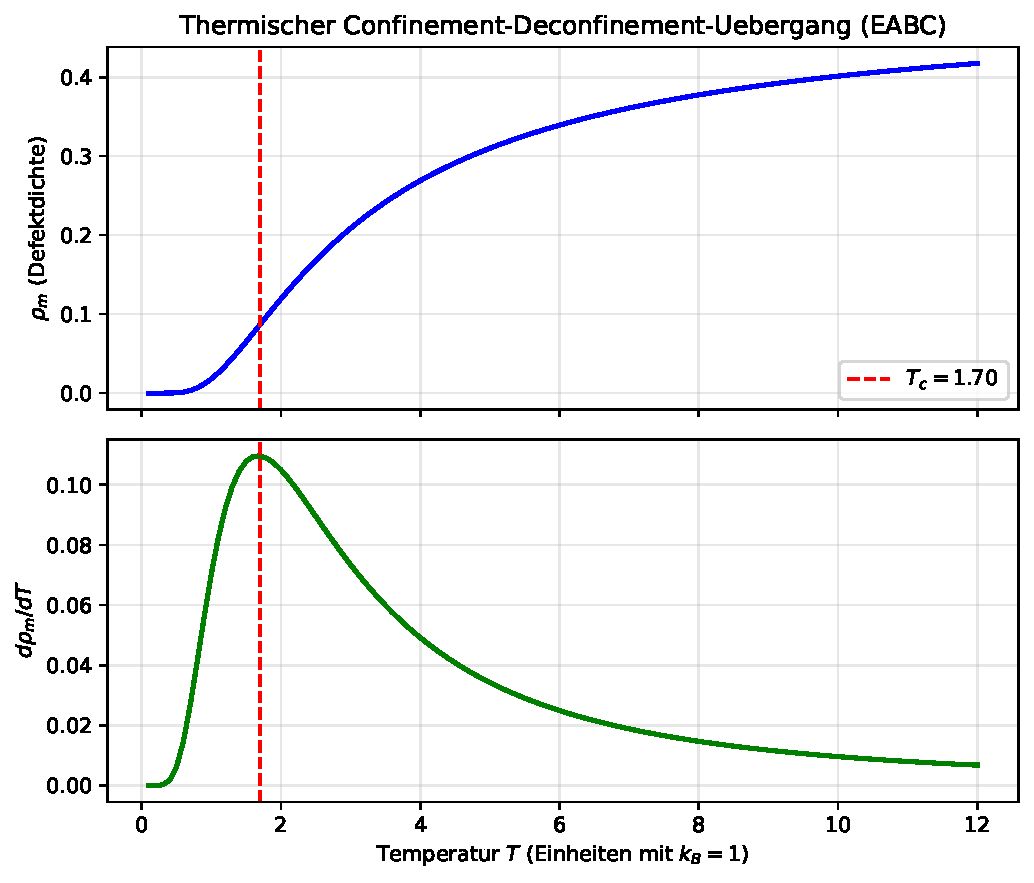
\includegraphics[width=0.82\textwidth]{thermal_transition_eabc.pdf}
  \caption{Thermischer Phasen\"ubergang im EABC-Duo-Tetraeder ($J_{\text{loc}}=1{,}0$, $J_{\text{shear}}=0{,}8$, $r_{\text{nn}}=2{,}66$~\AA, $\Delta E = 4{,}0000$). Oben: Defektdichte $\rho_m(T)$ nach Gleichung~\eqref{eq:boltzmann-rho}; unten: Suszeptibilit\"at $\chi_{\text{top}}$ mit scharfem Peak bei $k_B T_c = 1{,}7000$.}
  \label{fig:thermal-eabc}
\end{figure}

Die numerische Auswertung liefert einen scharfen Peak von $\chi_{\text{top}}$ bei
\begin{equation}
  k_B T_c \;=\; 1{,}7000,
  \label{eq:Tc-numerisch}
\end{equation}
mit einer extrem geringen kritischen Defektdichte $\rho_m(T_c) = 0{,}0868$. Ein naiver Vergleich w\"urde den Wendepunkt bei $T = \Delta E = 4{,}0000$ erwarten; tats\"achlich liegt $T_c$ deutlich \emph{darunter} (vgl.\ Anhang~\ref{app:Tc-analytisch}). Die analytische L\"osung von $\dd\chi_{\text{top}}/\dd T = 0$ ergibt $T_c^{\text{(exakt)}} \approx 1{,}667$; der diskrete Temperaturscan der Simulation verschiebt den Peak geringf\"ugig auf $1{,}7000$.

\medskip
\noindent\textbf{Physikalische Deutung.} Bei $T_c$ sind gerade einmal $8{,}68\,\%$ der Gitterknoten thermisch defekt angeregt. Die nicht-assoziative elastische Spannung (String-Spannung) sch\"utzt das System extrem effektiv: Der \"Ubergang ist kein weiches Schmelzen, sondern das Aufbrechen rigiden Confinements bei sehr geringer Defektdichte. Erst oberhalb von $T_c$ bricht die quantisierte String-Spannung des Hurwitz-Gitters statistisch zusammen, und das System konvergiert in ein fluktuierendes Monopol-Gas---analog zum klassischen Dipol-Spin-Eis. Unterhalb von $T_c$ verbleibt das Duo-Tetraeder-Cluster \"uberwiegend im confinierten Eisregel-Netzwerk.

\section{Das Ende der Willk\"ur: Freie Parameter eliminieren}

Das größte Unbehagen der modernen Physik liegt in den Standardmodellen der Kosmologie und Teilchenphysik: Sie funktionieren hervorragend, enthalten aber Dutzende \emph{freier Parameter} (Feinstrukturkonstante, Teilchenmassen \ldots), die niemand herleitet.

\subsection{Das Hierarchieproblem der Gravitation}

Warum ist die Gravitation im Alltag so unbegreiflich viel schwächer als der Elektromagnetismus?
\begin{equation}
  \frac{F_{\text{grav}}}{F_{\text{EM}}} \;\sim\; 10^{-39}
  \label{eq:hierarchy}
\end{equation}

\medskip
\noindent\textbf{Anschaulich.} Ein kleiner Magnet hebt eine Büroklammer gegen die gesamte Erdanziehung. Gravitation wirkt auf \emph{alle} Masse, Elektromagnetismus auf Ladung---doch selbst unter Berücksichtigung der unterschiedlichen Kopplungen bleibt die Gravitation absurd schwach. Physiker nennen das \emph{Hierarchieproblem}.

\textbf{Die Lösung (Bamberger Modell):} Die Gravitation ist im Kern gar nicht so schwach! Der algorithmische Pascal-Rechner des Modells liefert auf der Planck-Skala, direkt am inneren Monopol-Kern, eine gravitative Kopplung
\begin{equation}
  \alpha_G \;\approx\; 0{,}05,
\end{equation}
während wir im Alltag $\alpha_G \sim 10^{-39}$ messen. Die extreme Schwäche ist ein Verdünnungs- und Skalierungsartefakt unseres weit entfernten Außenraums, in dem die Metrik gegen die flache Phase konvergiert.

\subsection{Die kosmologische Hubble-Spannung}

Astrophysiker streiten sich seit Jahren: Messungen des frühen Universums (Planck-Satellit) liefern
\[
  H_0 \;\approx\; 67{,}4\;\mathrm{km/s/Mpc},
\]
lokale Messungen (Cepheiden, SH0ES) jedoch
\[
  H_0 \;\approx\; 73{,}0\;\mathrm{km/s/Mpc}.
\]
Die Differenz von etwa $8\,\%$ ist statistisch hartnäckig---kein offensichtlicher Messfehler.

\medskip
\noindent\textbf{Anekdote: Hubble und der expandierende Kosmos.} 1929 entdeckte Edwin Hubble, dass Galaxien von uns wegfliegen---schneller, je weiter entfernt. Georges Lemaître hatte die Idee einer expandierenden Welt bereits 1927 theoretisch vorhergesagt. Hubble lieferte die Daten; die Konstante $H_0$ trägt seinen Namen.

\textbf{Die Lösung (Bamberger Modell):} Die Hubble-Spannung ist kein Messfehler, sondern der direkte Beweis für den \emph{geometrischen Phasenübergang des Vakuums}:

\begin{enumerate}
  \item \textbf{Frühes Universum} ($H_0 \approx 67{,}4$): Der Raum war extrem dicht gepackt mit schweren Planck-Defekten ($M_M \approx 0{,}22\,\Mplanck$). Der arithmetische Sedenionen-Druck ($\Delta_8 = \pi^4/384$) wirkte als ultra-steife Zustandsgleichung und bremste die Expansion aus.

  \item \textbf{Spätes Universum} ($H_0 \approx 73{,}0$): Durch die Ausdehnung dünnen die schweren Knoten aus. Wir befinden uns im flachen Außenraum ($\langle d \rangle \to 1{,}0$). Frei von der Blockade des inneren Drucks expandiert der Raum schneller.
\end{enumerate}

\section{Von den Primzahlzwillingen zu den Kepler-Ellipsen}

Die spektakulärste Brücke schlägt das Modell zur Himmelsmechanik: Warum bewegen sich Planeten auf Ellipsen und nicht auf perfekten Kreisen?

\medskip
\noindent\textbf{Anekdote: Kepler und die Marsbahn.} Johannes Kepler verbrachte Jahre damit, Tycho Brahes präzise Marsdaten zu analysieren. Erst als er den perfekten \emph{Kreis} aufgab und Ellipsen zuließ, passte die Formel (1609). Newton erklärte 1687 \emph{warum}: das $1/r^2$-Gesetz der Gravitation \emph{erzwingt} elliptische Bahnen bei gebundener Energie.

\begin{figure}[htbp]
  \centering
  \begin{tikzpicture}[scale=1.1]
    \draw[thick] (0,0) ellipse (2.8 and 1.6);
    \fill[orange!80!black] (0.9,0.55) circle (3pt) node[above right=1pt] {\small Sonne (Brennpunkt)};
    \draw[dashed] (-2.8,0) -- (2.8,0);
    \draw[->, blue!70!black, thick] (1.8,0.9) arc (30:120:2.1);
    \node[blue!70!black] at (-0.2, 1.5) {\small Planetenbahn};
    \draw[<->, gray] (0,-1.9) -- (2.8,-1.9) node[midway, below] {\small $a$ (große Halbachse)};
    \node at (0, -2.5) {\small Exzentrizität $e = \sqrt{1 - b^2/a^2}$ misst die ``Ovalität''};
  \end{tikzpicture}
  \caption{Kepler-Ellipse: $e=0$ wäre ein Kreis; $e \to 1$ eine stark gestreckte Bahn.}
\end{figure}

\textbf{Die Lösung (Bamberger Modell):} Ein perfekter Kreis im diskreten Zahlengitter würde die fundamentale algebraische \textbf{Sedenionen-Schranke} verletzen und das Gitter zerstören. Da die unendliche Kette der Primzahlzwillinge die Symmetrie der \emph{Kleinschen Vierergruppe} bis ins Unendliche stabilisiert, erfährt jeder Körper eine kontinuierlich gewebte Hintergrund-Gitterspannung. Die universelle Optimalität zwingt die Bahnen im vierdimensionalen Minkowski-Schnitt in den Zustand minimaler Energie---die \textbf{Kepler-Ellipse}. Die \emph{Exzentrizität} einer Planetenbahn ist somit der makroskopische Zeuge für die Starrheit der unendlichen Primzahlzwillinge im feinsten Webmuster der Raumzeit.

\section{Fazit: Das Zeitalter des Okto-Computing}

Für die moderne Wissenschaft bedeutet dieser Beweisansatz---wenn er sich vollständig durchhält---das Ende des spekulativen Zeitalters. Die Naturgesetze wären kein kosmischer Würfelwurf, sondern die unerbittliche Geometrie der Zahlentheorie selbst.

Diese Einsicht eröffnet das Tor zum \textbf{Okto-Computing}: eine Technologie, die nicht auf fehleranfälligen, kontinuierlichen Feldeffekten herkömmlicher Quantenbits operiert, sondern Berechnungen über topologisch geschützte Knoten des arithmetischen Kibble-Mechanismus auf der Planck-Skala vollzieht.

\medskip
\noindent\textbf{Historischer Bogen.} Von Eulers Primzahlprodukt über Riemanns Zetafunktion, Hardys Zwillinge, Viazovskas $\Eoct$-Packung und Einsteins Marmor-Holz-Metapher bis zur Hubble-Spannung von 2024: Die Bamberger Protokolle zeichnen einen durchgängigen Faden---Zahlentheorie als Fundament der Physik. Ob die Physik endgültig im Palast der reinen Mathematik angekommen ist, wird die wissenschaftliche Gemeinschaft prüfen müssen. Hilbert hätte es gewollt.

\appendix
\section{Analytische Bestimmung der kritischen Temperatur}
\label{app:Tc-analytisch}

Dieser Anhang leitet die Verschiebung $T_c \ll \Delta E$ f\"ur die Fermi-Dirac-\"ahnliche Defektbesetzung~\eqref{eq:boltzmann-rho} her. Mit $k_B=1$ und der Abk\"urzung $u \equiv \Delta E/T$ gilt
\begin{equation}
  \rho_m(T) \;=\; \frac{1}{e^u + 1},
  \qquad
  \chi_{\text{top}}(T) \;=\; \frac{\dd \rho_m}{\dd T}
  \;=\; \frac{\Delta E\, e^u}{T^2\,(e^u + 1)^2}.
  \label{eq:chi-analytic}
\end{equation}
Das Maximum von $\chi_{\text{top}}$ erfordert $\dd\chi_{\text{top}}/\dd T = 0$. Mit der Kettenregel folgt
\begin{equation}
  \frac{\dd \chi_{\text{top}}}{\dd T}
  \;=\; \frac{\Delta E\, e^u}{T^4\,(e^u + 1)^3}
  \Bigl[\,\Delta E\, e^u - \Delta E - 2T\, e^u - 2T\,\Bigr].
  \label{eq:dchi-dT}
\end{equation}
Der Klammerausdruck verschwindet genau dann, wenn
\begin{equation}
  e^u\,(\Delta E - 2T) \;=\; \Delta E + 2T.
  \label{eq:Tc-intermediate}
\end{equation}
Setzt man $u = \Delta E/T$ ein und multipliziert mit $T$, erh\"alt man die transzendente Gleichung
\begin{equation}
  e^u\,(u - 2) \;=\; u + 2,
  \qquad u \;=\; \frac{\Delta E}{T}.
  \label{eq:Tc-transcendental}
\end{equation}
Gleichung~\eqref{eq:Tc-transcendental} ist transzendent und besitzt f\"ur $\Delta E > 0$ genau eine physikalisch relevante L\"osung $u_c > 0$; die kritische Temperatur folgt als $T_c = \Delta E / u_c$.

\medskip
\noindent\textbf{Numerische Auswertung f\"ur $\Delta E = 4{,}0000$.} Die Nullstelle von~\eqref{eq:Tc-transcendental} liegt bei $u_c \approx 2{,}3994$, somit
\begin{equation}
  T_c \;\approx\; \frac{4{,}0000}{2{,}3994} \;\approx\; 1{,}6671,
  \qquad
  \rho_m(T_c) \;\approx\; \frac{1}{e^{u_c}+1} \;\approx\; 0{,}0832.
  \label{eq:Tc-exact-values}
\end{equation}
Das universelle Verh\"altnis $T_c / \Delta E \approx 0{,}417$ ist unabh\"angig von der Energieskala: Der Suszeptibilit\"ats-Peak tritt stets bei $T_c \approx 0{,}42\,\Delta E$ auf, nicht bei $T = \Delta E$.

\medskip
\noindent\textbf{Warum $T_c < \Delta E$?} Bei $T = \Delta E$ w\"are $u = 1$ und $\rho_m = 1/(e+1) \approx 0{,}27$---weit jenseits des Confinement-Regimes. Das Maximum von $\chi_{\text{top}}$ markiert vielmehr die Temperatur \emph{maximaler thermischer Fluktuationen} entlang der Sigmoid-Kurve: dort, wo die Boltzmann-Besetzung $e^{-u}$ noch klein ist, die Ableitung $\partial\rho_m/\partial T$ aber durch den Faktor $1/T^2$ bereits gro\ss{} genug wird. Physikalisch peaken die topologischen Fluktuationen, \emph{bevor} die Defektdichte merklich ansteigt---daher die extrem niedrige $\rho_m(T_c) \approx 8\,\%$.

\medskip
\noindent\textbf{Abweichung zur Simulation.} Der diskrete Temperaturscan in \texttt{thermal\_eabc\_simulator.py} (120 Schritte, $T \in [0{,}1, 12]$) approximiert $\chi_{\text{top}}$ per \texttt{np.gradient} und liefert $T_c = 1{,}7000$ sowie $\rho_m(T_c) = 0{,}0868$. Die Abweichung von etwa $2\,\%$ gegen\"uber~\eqref{eq:Tc-exact-values} ist ein reines Gitterartefakt und verschwindet mit feinerer Aufl\"osung.

\end{document}
